\chapter{Identity Mixer}

Camenisch and Lysyanskaya~\cite{CamenischLysyanskaya2002,Lysyanskaya2002}
present a provably secure signature scheme and provide protocols for
\begin{enumerate}
  \item issuing a signature on a committed value, that is, blind
    signatures~\cite{Chaum1983}, and
  \item proving knowledge of a signature (on a committed value).
\end{enumerate}
This makes this scheme a suitable building block for privacy-preserving
technologies like anonymous credential systems.

Identity Mixer (Idemix)~\cite{IdemixCrypto2012} is an attribute-based
credential system developed at IBM Research Z\"urich. The core of this system is
the Camenisch-Lysyanskaya signature
scheme~\cite{CamenischLysyanskaya2002,Lysyanskaya2002} which allows multiple
messages to be signed at once. This allows a number of attributes to be combined
into a credential. In contrast to the U-Prove technology an Idemix credential
can be randomised (like the self-blindable credentials) allowing it to be used
multiple times while remaining anonymous.

In this chapter we focus on the core features of the Identity Mixer system:
credential issuance and selective disclosure of attributes. The technology
offers many more features that might be interesting to users of an
attribute-based credential system, but we focus on what can be achieved on a
smart card with an acceptable performance~\cite{VullersAlpar2013}. Additional
options can still be added, but at the cost of an increased transaction time.

\section{Camenisch-Lysyanskaya Signature Scheme}


This description is based on the Direct Anonymous Attestation explanation by
Camenisch~\cite{Camenisch2007} and the specification of the Identity Mixer
cryptographic library~\cite{IdemixCrypto2012}. These documents incorporate
improvements over the original scheme~\cite{CamenischLysyanskaya2002} presented
by Brickell, Camenisch, and Chen~\cite{BrickellCC2004} and by Camenisch and
Groth~\cite{CamenischGroth2004}.

\subsection{Key Generation}\label{sec:cl_keygen}

The public key consists of a special RSA modulus $n = p \cdot q$ where
$p = 2p' + 1$ and $q = 2q' + 1$ are safe primes. The private key in this scheme
are the primes $p'$ and $q'$. Furthermore we need a number of elements from the
group of quadratic residues modulo $n$,
$QR_n = \{ x : x,y \in \mathbb{Z}_n \land x \equiv y^2 \mod n \}$, in which
the computations take place:
\begin{itemize}
  \item $S$ with order $\#QR_n = p'q'$, is a generator of $QR_n$, and
  \item $Z$ $= S^{x_z} \mod n$ where $x_z \in_R [2, p'q' - 1]$ is an
    auxiliary value such that all computations remain within
    $\langle S \rangle$, the subgroup of $QR_n$ generated by $S$.
  \item Finally, for each message to be signed we need a base
    $R_i = S^{x_i} \mod n$ where $x_i \in_R [2, p'q' - 1]$.
\end{itemize}
Hence the resulting public key is $(n, S, Z, R_1, \dots, R_L)$ where $L$ is the
number of messages supported by this key.

In order to guarantee that such a public key has been constructed correctly,
that is, all values are elements of $\langle S \rangle$, a proof of
correctness can be constructed (Algorithm~\ref{alg:CL-proof-key}, based
on~\cite[Appendix A]{BrickellCC2004}):
\begin{multline*}
  SPK \{ (\alpha_z, \alpha_1, \dots, \alpha_L) : \\
  \bigwedge_{i = 1}^{L} R_i \equiv S^{\alpha_i} \mod n
  \quad\land\quad
  Z \equiv S^{\alpha_z} \mod n
  \} (n, R_1, \dots, R_L, S, Z)
\end{multline*}

This proof requires the use of binary challenges due to the security proof for
zero-knowledge. Hence, we need to generate commitments and responses for each
bit of the challenge $c$ which has length $l_H$, the output length of the hash
function.
% Special soundness: take two runs with the same commitment, but different
% challenges (and responses): (a, c, r) and (a, c', r').
%
% This gives y = g^{(r-r')/(c-c')}, hence witness w = (r-r')/(c-c').
% This can only be computed if:
% 1) c, c' are binary, thus delta(c) = +/- 1, or
% 2) under SRSA: delta(c) | delta(r) allows integer division
%       not(delta(c) | delta(r)) breaks SRSA, that is, it gives a root of g:
%            y^delta(c) = g^delta(r)    1 = a.delta(r) + b.delta(c)
%            g = g^{a.delta(r)} g^{b.delta(c)}
%              = y^{a.delta(c)} g^{b.delta(c)}
%              = (g^b y^a)^delta(c)
%
% The issuer knows the factorisation of n, and hence the order of the group, so
% SRSA does not hold in this case, so binary challenges is the only option here.

\begin{algorithm}
  \caption{Proof correctness of a Camenisch-Lysyanskaya public key.}
  \label{alg:CL-proof-key}
  \addtolength{\baselineskip}{1mm}
  \begin{algorithmic}[1]
    \Function{CL-proof-key}{$(n, S, Z, R_1, \dots, R_L)$}
      \ForAll{$j \in \{1, \dots, l_H\}$}
        \State $u_j \gets \Call{Random}{}$
        \State $Z'_j = S^{u_j} \mod n$
        \ForAll{$i \in \{1, \dots, L\}$}
          \State $v_{(i,j)} \gets \Call{Random}{}$
          \State $R'_{(i,j)} = S^{v_{(i,j)}} \mod n$
        \EndFor
      \EndFor

      \State $c \gets \Call{Hash}{n, S, Z, R_i, Z'_j, R'_{(i,j)}}$
        \Comment{for $1 \leq i \leq L$ and $1 \leq j \leq l_H$}

      \ForAll{$j \in \{1, \dots, l_H\}$}
        \State $r_j = u_j - c_j x_z \mod p'q'$
          \Comment{where $c_j$ is the $j$-th bit of $c$}
        \ForAll{$i \in \{1, \dots, L\}$}
          \State $s_{(i,j)} \gets v_{(i,j)} - c_j x_i \mod p'q'$
            \Comment{where $c_j$ is the $j$-th bit of $c$}
        \EndFor
      \EndFor

      \Return $(c, r_j, s_{(i,j)})$
        \Comment{for $1 \leq i \leq L$ and $1 \leq j \leq l_H$}
    \EndFunction
  \end{algorithmic}
\end{algorithm}

The proof can be verified using Algorithm~\ref{alg:CL-verify-key}, which
reconstructs the input of the hash based on the proof values and then checks
whether the output of the hash matches the given value. These values can be
reconstructed because:
\begin{equation*}
  Z^{c_j} \cdot S^{r_j}
  \equiv (S^{x_z})^{c_j} \cdot S^{r_j}
  \equiv (S^{x_z})^{c_j} \cdot S^{u_j - c_j x_z}
  \equiv S^{u_j}
  \equiv Z'_j \mod n \text{, and}
\end{equation*}
\begin{equation*}
  R_i^{c_j} \cdot S^{s_{(i,j)}}
  \equiv (S^{x_i})^{c_j} \cdot S^{s_{(i,j)}}
  \equiv (S^{x_i})^{c_j} \cdot S^{v_{(i,j)}-c_j x_i}
  \equiv S^{v_{(i,j)}}
  \equiv R'_{(i,j)} \mod n \text{.}
\end{equation*}

\begin{algorithm}[t]
  \caption{Verify correctness of a Camenisch-Lysyanskaya public key.}
  \label{alg:CL-verify-key}
  \addtolength{\baselineskip}{1mm}
  \begin{algorithmic}[1]
    \Function{CL-verify-key}{$(n, S, Z, R_1, \dots, R_L), (c, r_j, s_{(i,j)})$}
      \ForAll{$j \in \{1, \dots, l_H\}$}
        \State $Z'_j \gets Z^{c_j} \cdot S^{r_j} \mod n$
          \Comment{where $c_j$ is the $j$-th bit of $c$}
        \ForAll{$i \in \{1, \dots, L\}$}
          \State $R'_{(i,j)} \gets R_i^{c_j} \cdot S^{r_{(i,j)}} \mod n$
            \Comment{where $c_j$ is the $j$-th bit of $c$}
        \EndFor
      \EndFor

      \State $c' \gets \Call{Hash}{n, S, Z, R_i, Z'_j, R'_{(i,j)}}$
        \Comment{for $1 \leq i \leq L$ and $1 \leq j \leq l_H$}

      \If{$c \neq c'$}
        \Return \Call{Invalid}{}
      \EndIf

      \Return \Call{Valid}{}
    \EndFunction
  \end{algorithmic}
\end{algorithm}

%As given in Section~\ref{sec:cl_blind-sign}. Alternatively as given in
%Section~\ref{sec:cl_basic-sign} with an additional proof that
%$A \in \langle S \rangle$. This can be derived from correct construction of the
%signature, together with the correct construction of the keys.

%$S \longrightarrow R$: $PK\{(\delta) : A \equiv \pm \left(\dfrac{Z}{U S^{v''}
%\prod_{i=L'+1}^{L} R_i^{m_i}} \right)^{\delta} \mod n \}$

\subsection{Basic Signature Scheme}\label{sec:cl_basic}

In order to sign a number of messages $m_1, \dots, m_L$, they first have to be
aggregated into a single group element $Q$ according to~(\ref{eqn:CL-aggregate})
where $v$ is a random number (used to randomise the signature and when blinding
the messages, see Section~\ref{sec:cl_blind}).
\begin{equation}\label{eqn:CL-aggregate}
  Q \equiv \dfrac{Z}{S^v \prod_{i=1}^{L} R_i^{m_i}} \mod n
\end{equation}
Next a random prime $e$ is generated which is used as an ephemeral RSA public
key for this signature. Finally, $A = Q^d \mod n$ is an RSA signature over the
aggregated messages where $d = e^{-1} \mod (p' \cdot q')$ is the RSA private
key corresponding to $e$. As a result the signature over the messages
$m1, \dots, m_L$ is the tuple $(A, e, v)$ (see Algorithm~\ref{alg:CL-sign}).

\begin{algorithm}
  \caption{Generate a basic Camenisch-Lysyanskaya signature.}
  \label{alg:CL-sign}
  \addtolength{\baselineskip}{1mm}
  \begin{algorithmic}[1]
    \Function{CL-sign}{$m_1, \dots, m_L, (n, R_1, \dots, R_L, S, Z), (p', q')$}
      \State $v \gets \Call{Random}{}$
      \State $U \gets S^v \mod n$
      \ForAll{$i \in \{1, ..., L\}$}
        \State $U \gets U \cdot R_i^{m_i} \mod n$
      \EndFor
      \State $Q \gets Z \cdot U^{-1} \mod n$

      \State $e \gets \Call{RandomPrime}{}$
      \State $d \gets e^{-1} \mod (p' \cdot q')$
      \State $A \gets Q^d \mod n$

      \Return $(A, e, v)$
    \EndFunction
  \end{algorithmic}
\end{algorithm}

To verify this Camenisch-Lysyanskaya signature the RSA signature over the
aggregated messages has to be verified, that is, the following equation has to
be checked:
\begin{equation*}
  A^e \equiv \dfrac{Z}{S^v \prod_{i=1}^{L} R_i^{m_i}} \mod n
\end{equation*}
This is equivalent to checking the following equation, as used in
Algorithm~\ref{alg:CL-verify}:
\begin{equation*}
  Z \equiv A^e S^v \prod_{i=1}^{L} R_i^{m_i} \mod n
\end{equation*}

\begin{algorithm}
  \caption{Verify a basic Camenisch-Lysyanskaya signature.}
  \label{alg:CL-verify}
  \addtolength{\baselineskip}{1mm}
  \begin{algorithmic}[1]
    \Function{CL-verify}{$m_1, \dots, m_L, (A, e, v), (n, R_1, \dots, R_L, S, Z)$}
      \State $Z' \gets A^e \cdot S^v \mod n$
      \ForAll{$i \in \{1, ..., L\}$}
        \State $Z' \gets Z' \cdot R_i^{m_i} \mod n$
      \EndFor

      \If{$Z \neq Z' \mod n$}
        \Return \Call{Invalid}{}
      \EndIf

      \Return \Call{Valid}{}
    \EndFunction
  \end{algorithmic}
\end{algorithm}

%\paragraph{Verify} the following for a signature $(e, v, A)$ on messages $m_1, \dots, m_L$
%\begin{equation*}
%  Z \equiv A^e S^v \prod_{i=1}^{L} R_i^{m_i} \mod n
%  \quad\land\quad
%  \bigwedge_{i=1}^{L} m_i \in \pm \{0,1\}^{l_m}
%  \quad\land\quad
%  2^{l_e-1} < e < 2^{l_e}
%\end{equation*}

\subsection{Blind signatures}\label{sec:cl_blind}

\begin{figure}
  \centering
  \includegraphics[scale=.45]{mscs/cl_blind-sign_simple}
  \caption{Blind signature generation}
  \label{msc:cl_blind-sign}
\end{figure}

%\begin{figure}
%  \centering
%  \includegraphics[scale=.45]{mscs/cl_blind-sign_pku}
%  \caption{$PK\{(\mu_1, \dots, \mu_{L'}, \nu') :
%    U \equiv \pm S^{\nu'} \prod_{i=1}^{L'} R_i^{\mu_i} \mod n \;\land\; \mu_1, \dots, \mu_{L'} \in \pm\{0,1\}^{l_m} \}$}
%  \label{msc:cl_blind-sign_pku}
%\end{figure}

%\begin{figure}
%  \centering
%  \includegraphics[scale=.45]{mscs/cl_blind-sign_pka}
%  \caption{$PK\{(\delta) :
%  A \equiv \pm \left(\dfrac{Z}{U S^{v''} \prod_{i=L'+1}^{L} R_i^{m_i}} \right)^{\delta} \mod n \}$}
%  \label{msc:cl_blind-sign_pka}
%\end{figure}

\begin{algorithm}
  \caption{Prepare for a blind Camenisch-Lysyanskaya signature.}
  \label{alg:CL-blind-prepare}
  \addtolength{\baselineskip}{1mm}
  \begin{algorithmic}[1]
    \Function{CL-blind-prepare}{$m_1, \dots, m_L', (n, S, Z, R_1, \dots, R_L)$}
      \State $v' \gets \Call{Random}{}$
      \State $U \gets S^{v'}$
      \ForAll{$i \in \{1, ..., L'\}$}
        \State $U \gets U \cdot R_i^{m_i} \mod n$
      \EndFor

      \Return $(U, v')$
    \EndFunction
  \end{algorithmic}
\end{algorithm}

\begin{algorithm}
  \caption{Generate a proof of correctness for $U$.}
  \label{alg:CL-proof-U}
  \addtolength{\baselineskip}{1mm}
  \begin{algorithmic}[1]
    \Function{CL-proof-U}{$(U, v'), n_U, m_1, \dots, m_L', (n, S, Z, R_1, \dots, R_L)$}
      \State $u \gets \Call{Random}$
      \State $a \gets S^u$
      \ForAll{$i \in \{1, ..., L\}$}
        \State $v_i \gets \Call{Random}$
        \State $a \gets R_i^{v_i} \mod n$
      \EndFor
      \State $c \gets \Call{Hash}{U, a, n_U}$
      \State $r \gets u + c \cdot v'$
      \ForAll{$i \in \{1, ..., L'\}$}
        \State $s_i \gets v_i + c \cdot m_i$
      \EndFor

      \Return $(a, r, s_1, \dots, s_L')$
    \EndFunction
  \end{algorithmic}
\end{algorithm}

\begin{algorithm}
  \caption{Verify the proof of correctness for $U$.}
  \label{alg:CL-verify-U}
  \addtolength{\baselineskip}{1mm}
  \begin{algorithmic}[1]

    \Function{CL-verify-U}{$U, (a, r, s_1, \dots, s_L'), n_U, (n, R_1, \dots, R_L, S, Z)$}
      \State $c \gets \Call{Hash}{U, a, n_U}$
      \State $U' \gets S^r \mod n$
      \ForAll{$i \in \{1, ..., L'\}$}
        \State $U' \gets U' \cdot R_i^{s_i} \mod n$
      \EndFor
      \If{$U' \neq a \cdot U^c \mod n$}
        \Return \Call{Invalid}{}
      \EndIf

      \Return \Call{Valid}{}
    \EndFunction
  \end{algorithmic}
\end{algorithm}

\begin{algorithm}
  \caption{Generate a blind Camenisch-Lysyanskaya signature.}
  \label{alg:CL-blind-sign}
  \addtolength{\baselineskip}{1mm}
  \begin{algorithmic}[1]

    \Function{CL-sign}{$U, m_{L'+1}, \dots, m_L, (n, R_1, \dots, R_L, S, Z), (p', q')$}
      \State $v'' \gets \Call{Random}{}$
      \State $U \gets U \cdot S^{v''} \mod n$
      \ForAll{$i \in \{L' + 1, ..., L\}$}
        \State $U \gets U \cdot R_i^{m_i} \mod n$
      \EndFor
      \State $Q \gets Z \cdot U^{-1} \mod n$

      \State $e \gets \Call{RandomPrime}{}$
      \State $d \gets e^{-1} \mod (p' \cdot q')$
      \State $A \gets Q^d \mod n$

      \Return $(A, e, v''), (c', r')$
    \EndFunction
  \end{algorithmic}
\end{algorithm}

\begin{algorithm}
  \caption{Generate a proof of correctness or $A$.}
  \label{alg:CL-proof-A}
  \addtolength{\baselineskip}{1mm}
  \begin{algorithmic}[1]
    \Function{CL-proof-A}{$(A, e, v), n_A, (n, R_1, \dots, R_L, S, Z), (p', q')$}
      \State $u \gets \Call{Random}{}$
      \State $a \gets Q^u \mod n$
      \State $c \gets \Call{Hash}{A, a, n_A}$
      \State $r \gets u - c \cdot e^{-1} \mod (p' \cdot q')$

      \Return $(c, r)$
    \EndFunction
  \end{algorithmic}
\end{algorithm}

\begin{algorithm}
  \caption{Verify the proof of correctness for $A$.}
  \label{alg:CL-verify-A}
  \addtolength{\baselineskip}{1mm}
  \begin{algorithmic}[1]
    \Function{CL-verify-A}{$v', (A, e, v'')$}
      \If{}
        \Return \Call{Invalid}{}
      \EndIf
      \Return \Call{Valid}{}
    \EndFunction
  \end{algorithmic}
\end{algorithm}

\begin{algorithm}
  \caption{Finish a blind Camenisch-Lysyanskaya signature.}
  \label{alg:CL-blind-finish}
  \addtolength{\baselineskip}{1mm}
  \begin{algorithmic}[1]
    \Function{CL-blind-finish}{$v', (A, e, v'')$}
      \LineComment{Construct the final signature}
      \State $v \gets v' + v''$

      \Return $(A, e, v)$
    \EndFunction
  \end{algorithmic}
\end{algorithm}

\paragraph{Output} signature $(e, v, A)$ as depicted in Figure~\ref{msc:cl_blind-sign}, whereas the zero-knowledge protocols are given in Figures~\ref{msc:cl_blind-sign_pku} and~\ref{msc:cl_blind-sign_pka} respectively.

%$R$: $v' \in_R \{0,1\}^{l_n+l_\varnothing}; U = S^{v'} \prod_{i=1}^{L'} R_i^{m_i} \mod n$ \\
%$R \longrightarrow S$: $U, PK\{(\mu_1, \dots, \mu_{L'}, \nu') : U \equiv \pm S^{\nu'} \prod_{i=1}^{L'} R_i^{\mu_i} \mod n \land \mu_1, \dots, \mu_{L'} \in \pm\{0,1\}^{l_m} \}$ \\
%$S$: $\hat{v} \in_R \{0,1\}^{l_v-1}; e \in_R [2^{l_e-1} + 1, 2^{l_e} -1]; v'' = \hat{v} + 2^{l_v - 1}; A = \left(\dfrac{Z}{U S^{v''}\prod_{i=L'+1}^{L} R_i^{m_i}} \right)^{1/e} \mod n$ \\
%$S \longrightarrow R$: $(A, e, v''), PK\{(\delta) : A \equiv \pm \left(\dfrac{Z}{U S^{v''} \prod_{i=L'+1}^{L} R_i^{m_i}} \right)^{\delta} \mod n \}$ \\
%$R$: verify $e \in [2^{l_e-1} + 1, 2^{l_e} -1]$ is prime; $v = v' + v''$


\subsection{Signature proving}\label{sec:cl_proof}


\paragraph{Input} elements $g_1, \dots, g_L$ where
\begin{description}
  \item[$g_1, \dots, g_L$] $\in G = \langle g_0 \rangle$ where $G$ is a group of prime order $q > 2^{l_m}$ generated by $g_0$
\end{description}

\paragraph{Output}

$R$: $r' \in \{0,1\}^{l_n + l_\varnothing}; C = g_0^{r'} \prod_{i \in I_c} g_i^{m_i}; r \in_R \{0, 1\}^{l_n + l_\varnothing}; A' = A S^r$ \\
$R \longrightarrow V$: $A', C, m_i$ where $i \not\in I_c \cup I_h$,
$PK\{ (\varepsilon, \tilde{\nu}, \rho', \{\mu_i : i \in I_c \cup I_h\}) :
Z A'^{-2^{l_e -1}} \prod_{i \not\in I_c \cup I_h} R_i^{-m_i} \equiv \pm A'^\varepsilon S^{\tilde{\nu}} \prod_{i \in I_c \cup I_h} R_i^{\mu_i} \mod n \land
C \equiv g_0^{\rho'} \prod_{i \in I_c} g_i^{\mu_i} \land
\bigwedge_{i \in I_c \cup I_h} \mu_i \in \{0,1\}^{l_m + l_\varnothing + l_H + 2} \land
\varepsilon \in \pm \{0,1\}^{l'_e + l_\varnothing | l_H + 1} \}$ \\
$V$: verify $m_i \in \pm \{0,1\}^{l_m}$ for $i \not\in I_c \cup I_h$

\section{Credential Verification}

\subsection{Randomisation}

The signature is randomised to prevent linkability based on the signature values $A, e, v$.
First a random blinding value $r_A$ is generated to randomise $A$.
Next the values $e$ and $v$ are adjusted such that the signature remains valid.

\begin{algorithm}[ht]
  \caption{Randomise the signature}
  \addtolength{\baselineskip}{1mm}

  \begin{algorithmic}[1]
    \item[\textbf{Parameters}] $n, S$

    \Statex
    \Function{RandomiseSignature}{$A$, $e$, $v$}
      \State $r_A \gets \Call{RandomBits}{\ell_{n} + \ell_{\o}}$
      \State $A' \gets A \cdot S^{r_A} \mod n$
      \State $e' \gets e - 2^{\ell_{e} - 1}$
      \State $v' \gets v - e \cdot r_A$
      \State \Return $A', e', v'$
    \EndFunction
  \end{algorithmic}
\end{algorithm}

Note that this randomisation operation only effectively randomises the $A$ value of the signature.
Hence it is required to hide the $e'$ and $v'$ using a zero-knowledge proof when revealing this randomised signature.


\subsection{Selective disclosure \& Zero-knowledge proof}

We can distinguish two types of credentials. A root credential which contains the special attributes $a_\mathtt{nym}$ and $a_\mathtt{rev}$, and regular credentials which do not contain these values. The root credential is used when a pseudonym and/or revocation check is required, whereas regular credentials are used to reveal attributes. This can also be combined, either by including attributes in the root credential, or using additional credentials besides the root credential.

All credentials contain the device master secret $s$ which binds the credential to the device. This secret should be stored in a protected manner to prevent cloning of the credentials to other devices. Furthermore, an attribute $a_\mathtt{exp}$ containing expiry information (general enough to prevent identification based on this value) is contained in each credential such that the validity of the credential can be verified. Therefore $a_\mathtt{exp}$ is always revealed during a selective disclosure proof. In contrast, the secret $s$ and attributes $a_\mathtt{nym}$ and $a_\mathtt{rev}$ are never revealed. Any other attributes contained by a credential are denoted as $a_1, \dots, a_l$, where $l$ is the number of attributes. The signature over the credential containing these attributes is the triplet $(A, e, v)$.

We assume that a (secure) session has been established and that any information relevant to this session is captured in the $\mathtt{context}$ variable. When a service provider needs a pseudonym and/or attributes a request is sent containing an attribute disclosure selection $\mathcal{D}$ to indicate which attributes should be revealed and a fresh $\mathtt{nonce}$ to ensure a freshly generated proof.

Algorithm~\ref{alg:proof} describes the operations that have to be performed to generate a selective disclosure proof, including pseudonym and revocation. The first step in this algorithm is to generate the pseudonym and revocation values as well as to randomise the signature. The next step is the zero-knowledge proof which hides the undisclosed attributes and the $e'$ and $v'$ values from the randomised signature. Furthermore this proof binds the pseudonym and revocation values to the signature to guarantee authenticity and correctness of the generated values.

The zero-knowledge proof is constructed in four steps. First a bunch of blinding values is generated to hide all values that are not revealed in this proof. The next step is to commit to these blinding values by calculating the commitments. These commitments are then used to generate the challenge which is the input to the final step, the calculation of the responses. Finally the proof, the challenge and the responses, together with the revealed values are returned.

\begin{algorithm}
  \caption{Prove the attributes}
  \label{alg:proof}
  \addtolength{\baselineskip}{1mm}
  \begin{algorithmic}[1]

    \item[\textbf{Card}] $s$
    \item[\textbf{Credential}] $a_\mathtt{exp}, a_{1 \dots l}, (n, S, Z, R_{s, \mathtt{exp}, 1 \dots l}), (A, e, v)$
    \item[\textbf{Session}] $\mathtt{context}$
    \item[\textbf{Request}] $\mathcal{D}, \mathtt{nonce}$

    \Statex
    \Function{GenerateProof}{}
      \State $A', e', v' \gets \Call{RandomiseSignature}{A, e, v}$

      \Statex \Comment{Generate all blinding values}
      \State $\tilde{e} \gets \Call{RandomBits}{\ell_{e'} + \ell_{\text{\o}} + \ell_{H}}$
      \State $\tilde{v} \gets \Call{RandomBits}{\ell_{v} + \ell_{\o} + \ell_{H}}$
      \State $\tilde{s} \gets \Call{RandomBits}{\ell_{m} + \ell_{\o} + \ell_{H}}$
      \ForAll{$i \notin \mathcal{D}$} \Comment{undisclosed attributes}
        \State $\tilde{a}_i \gets \Call{RandomBits}{\ell_{m} + \ell_{\o} + \ell_{H}}$
      \EndFor

      \Statex \Comment{Compute the commitment}
      \State $\tilde{Z} \gets {A'}^{\tilde{e}} \cdot S^{\tilde{v}} \cdot R_0^{\tilde{s}} \mod n$
      \ForAll{$i \notin \mathcal{D}$} \Comment{undisclosed attributes}
        \State $\tilde{Z} \gets \tilde{Z} \cdot R_i^{\tilde{a}_i} \mod n$
      \EndFor

      \Statex \Comment{Generate the challenge}
      \State $c \gets \Call{Hash}{\mathtt{context} || A' || \mathtt{ID_{nym}} || \mathtt{ID_{rev}} ||
        \tilde{Z} || \mathtt{nonce}}$

      \Statex \Comment{Compute the responses}
      \State $\hat{e} \gets \tilde{e} + c \cdot e'$
      \State $\hat{v} \gets \tilde{v} + c \cdot v'$
      \State $\hat{s} \gets \tilde{s} + c \cdot s$
      \ForAll{$i \notin \mathcal{D}$} \Comment{undisclosed attributes}
        \State $\hat{a}_i \gets \tilde{a}_i + c \cdot a_i$
      \EndFor

      \Statex
      \Return $c, A', \hat{e}, \hat{v}, \hat{s}, \hat{a}_\mathtt{nym}, \hat{a}_\mathtt{rev}, \hat{a}_{i \notin \mathcal{D}}, a_\mathtt{exp}, a_{i \in \mathcal{D}}$
    \EndFunction
  \end{algorithmic}
\end{algorithm}

\subsection{Verification}

Once a service provider receives the attributes $a_{i \in \mathcal{D}}$, the pseudonym $\mathtt{ID_{nym}}$ and device revocation value $\mathtt{ID_{rev}}$ it can just use those to provide its service. However, the proper solution is to first verify the proof generated by the card to assess the validity of these values.

The verification procedure is given in Algorithm~\ref{alg:verify}. This procedure starts with reconstructing the commitments using the responses (and the received challenge). Using these commitments the challenge can be reconstructed which can then be verified with the challenge value received from the card. If these challenges match, the proof is valid, otherwise it is invalid and the received values should not be used for any further processing (except perhaps for reporting this incident). Finally, the service provider should check the $a_{\mathtt{exp}}$ value to determine whether or not the credential has expired.

\begin{algorithm}
  \caption{Verify the attributes}
  \label{alg:verify}
  \addtolength{\baselineskip}{1.5mm}

  \begin{algorithmic}[1]
    \item[\textbf{Session}] $\mathtt{context}$
    \item[\textbf{Request}] $\mathcal{D}, \mathtt{nonce}$
    \item[\textbf{Response}] $c, A', \hat{e}, \hat{v}, \hat{s}, \hat{a}_\mathtt{nym}, \hat{a}_\mathtt{rev}, \hat{a}_{i \notin \mathcal{D}}, a_\mathtt{exp}, a_{i \in \mathcal{D}}$

    \Statex
    \Function{VerifyProof}{}
      \Statex \Comment{Reconstruct the commitments}
      \State $\hat{Z} \gets (A')^{2^{\ell_e - 1}} \cdot R_\mathtt{exp}^{a_\mathtt{exp}} \mod n$
      \ForAll{$i \in \mathcal{D}$} \Comment{disclosed attributes}
        \State $\hat{Z} \gets \hat{Z} \cdot R_i^{a_i} \mod n$
      \EndFor
      \State $\hat{Z} \gets \hat{Z}^c \cdot Z^{-c} \cdot (A')^{\hat{e}} \cdot S^{\hat{v}} \mod n$
      \ForAll{$i \notin \mathcal{D}$} \Comment{undisclosed attributes}
        \State $\hat{Z} \gets \hat{Z} \cdot R_i^{\hat{a}_i} \mod n$
      \EndFor
      \Statex \Comment{Reconstruct the challenge}
      \State $\hat{c} \gets \Call{Hash}{\mathtt{context} || A' || \mathtt{ID_{nym}} || \mathtt{ID_{rev}} ||
        \hat{Z} || \mathtt{nonce}}$
      \Statex \Comment{Verify the challenge}
      \If{$c = \hat{c}$}
        \Return \Call{Valid}{}
      \Else
        \Return \Call{Invalid}{}
      \EndIf
    \EndFunction
  \end{algorithmic}
\end{algorithm}



\section{Idemix on Smart Cards}

The main objective of our research is to assess how well privacy-friendly
protocols perform when run on a smart card. Hence implementing our prototypes
requires an open smart card platform that also provides the necessary
cryptographic hardware support. Previous
research~\cite{TewsJacobs09,MostowskiVullers11} clearly shows that purely
software based prototypes do not offer sufficient performance for realistic
use, while proper hardware support makes the prototypes practically usable. In
this case we used an Infineon SLE78 chip\footnote{This is the successor to the
Infineon SLE66 chip used by Mostowski and Vullers~\cite{MostowskiVullers11}.}
running the MULTOS platform. This platform offers an API which exposes the
(hardware supported) modular arithmetic operations required to implement
technologies like Idemix and U-Prove.

\subsection{System Architecture}

\begin{figure}[t]
  \centering
  \begin{subfigure}{0.45\textwidth}
    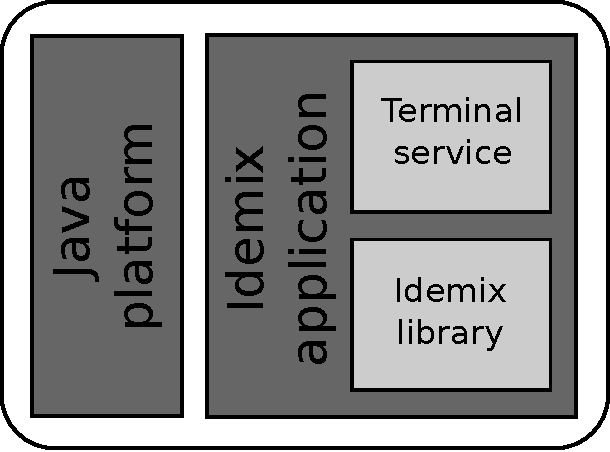
\includegraphics[scale=.45]{images/idemix-terminal-architecture}
    \caption{Terminal}
    \label{fig:terminal-architecture}
  \end{subfigure}
  \qquad
  \begin{subfigure}{0.45\textwidth}
    \includegraphics[scale=.45]{images/idemix-card-architecture}
    \caption{Card}
    \label{fig:card-architecture}
  \end{subfigure}
  \caption{System architecture for Idemix on a smart card.}
  \label{fig:architecture}
\end{figure}

Our system consists of two parts, depicted in Figure~\ref{fig:architecture}, a
terminal~\subref{fig:terminal-architecture} which interacts with a
card~\subref{fig:card-architecture} using APDUs. The terminal application is
written in Java and uses the Idemix cryptographic library\footnote{Available
for download at \url{https://prime.inf.tu-dresden.de/idemix/}} provided by IBM
Research. We created an extension to this library, the terminal service, which
takes care of all smart card specifics. The service implements the user roles
of the Idemix issuance and verification protocols, described by the
\texttt{Recipient} and \texttt{Prover} interfaces respectively. These
interfaces are implemented by translating all Java method calls from the
library into the corresponding APDU commands and converting the Java data types
to raw byte arrays, suitable for APDU communication.

The Idemix application on the card takes care of handling the incoming APDUs
and storing the values into the internal data structures. While handling the
communication with the terminal is the largest part of the application, the main
part is the implementation of the cryptographic operations for the Idemix
protocols. This allows the card to perform the user roles without depending on
the terminal for any computations or proof generation. The only thing the
terminal is responsible for is providing the data in the correct format.

\subsection{Smart Card Implementation}

Just as Mostowski and Vullers~\cite{MostowskiVullers11} with their U-Prove
implementation, we have chosen to use the MULTOS C interface to do our
prototype implementation of Idemix. The programming environment is convenient
for smart card programming and allows us some more flexibility for memory
management. It will be explained below why this is crucial.

Implementing the Idemix specification did not turn out to be that hard in the
beginning, the available API makes it easy to implement the cryptographic
protocol. In principle, it is a direct translation from the mathematical
description to API calls. The only API restriction we came across was that the
\texttt{ModularExponentiation} function does not accept exponents larger than
the modulus size. For Idemix this only involves exponentiations with base $S$
(see details in Section~\ref{sec:specIdemixTheory}). Hence we added a function
\texttt{SpecialModularExponentiation} which implements the same method as used
by Bichsel et al.~\cite{BichselCGS2009}, that is, splitting one exponentiation
up into two\footnote{This method actually requires three exponentiations, but
we can precompute one exponentiation during initialisation, since we only need
this method for the base $S$.} exponentiations and one multiplication.

Our initial implementation only used static memory to store the variables. This
allowed us to work without thinking about which memory segment to use. The
drawback of this approach was a bad performance caused by the EEPROM memory
which takes a long time, compared to RAM, to write new values.

Once we had a functionally correct implementation, we started to optimise. This
was done by moving the buffer, which stores the intermediate results for larger
computations, to the public memory. The next step was to move the session
variables to the dynamic memory, which required careful organisation due to the
limited amount of available storage. However, when the dynamic memory use
increased the stack-based execution model started to cause trouble.

Initially, the stack could use the full size of the dynamic memory, such that
we had sufficient space to use functions and put the (relatively) large input
values on the stack. When using the C-interface, the compiler takes care of
managing the stack and putting input values on it when an instruction needs
this. However, this makes it difficult to get an idea on how much space the
stack actually needs. By trial and error, we discovered that we used quite some
amount of memory for the stack, which left us with only limited amount of space
for session variables.

To improve this situation, we reduced the number of function calls by inlining
some convenience functions. We also switched to using global variables instead
of function parameters, such that when we use a function, it does not require
much space on the stack. To get the last few, often used, variables into RAM,
we decided to split up some computations into smaller parts such that the
values to be put on the stack also get smaller. For example, additions can be
computed using addition with carry, and multiplications using grade-school
multiplication. This adds a number of extra operations, but it is worth the
memory gain which results in improved performance.

Finally, we translated most parts of the cryptographic code to MEL assembly
which allowed us to optimise the use of stack and reduce the amount of memory
operations during calculations. This was required since the provided C-functions
moved the values from the stack to the variable locations, while they are needed
again in the next operation. By doing this we could reduce the amount of memory
required for intermediate values which in the end allowed us to get all
necessary variables in RAM.

The resulting code can be found in the \verb!idemix_multos! GitHub repository at
\url{https://github.com/credentials/}. The repositories listed at this page are
used within the IRMA project (\url{https://irmacard.org/}) which aims to develop
an infrastructure for using attribute-based credentials on smart cards. A pilot,
with government support, will be launched early 2013.

\section{Results and Comparison}

We mainly compare our results with the U-Prove implementation by Mostowski and
Vullers~\cite{MostowskiVullers11} as this implementation offers similar
functionality using the same modulus size (1024 bits) and the same platform.
During initial development we even used the same SLE66-based cards, but in the
end we managed to get newer SLE78-based cards which we currently use. For the
conclusions this makes no difference since already with our SLE66 optimised
prototype we got similar results, the SLE78 implementation only improved the
running times.

There are two important performance measures: the time it takes to issue a new
credential to the card, and the running time of the verification protocol.

\subsection{Credential Issuance}

\begin{figure}[b]
  \centering
  \includegraphics{images/idemix-graphs5.mps}

  \caption[Credential issuance times.]{
    Credential issuance times
    (\raisebox{-.8\dp\strutbox}{\includegraphics{images/idemix-graphs8.mps}}:~computations,
      \raisebox{-.8\dp\strutbox}{\includegraphics{images/idemix-graphs7.mps}}:~overhead; 1024 bits).}
  \label{fig:issuance}
\end{figure}

For issuance, we measured the running time of the protocol and determined how
much time was actually spent on computations and which part was used to transfer
and store the values (marked as overhead; see Figure~\ref{fig:issuance}). These
values offer a clear improvement over the U-Prove issuance times
from~\cite{MostowskiVullers11}, which take 3623 and 5489 ms for 2 and 5
attributes respectively. Not only are the absolute values better, the additional
time it takes to issue more attributes is less than with the U-Prove
implementation.

Sterckx et al.~\cite{Sterckx09} implement the Direct Anonymous Attestation (DAA)
protocol, which is derived from the Idemix protocols on a Java~Card. With a
1024 bits modulus they achieve a running time of 2.4 seconds of which 19\% is
overhead, which gives a computation time of approximately 1.9 seconds. This is
good, but unfortunately the DAA protocol does not support any attributes as it
is just targeted at anonymous authentication and hence only uses a secret key.

Bichsel et al.~\cite{BichselCGS2009} from the Idemix team at IBM Research
Z\"urch also implemented a variant of the DAA protocol on a Java~Card. They
report a running time of 7.4 seconds for a modulus size of 1280 bits, which is
larger than the 1024 bits we used. It is unclear, however, which transaction
time they measured. But again, this implementation does not include any
attributes.

\subsection{Selective Disclosure of Attributes}

For selective disclosure, we measured the running times of four configurations
(see Figure~\ref{fig:proving}). These configurations have been chosen because
two is the smallest number of attributes for which selective disclosure makes
sense and five is the largest number of attributes used in our pilot project.
By comparing these graphs, it is clear that each attribute that is not disclosed
adds roughly 100ms of computation time, whereas the amount of work per
undisclosed attribute remains the same.

\begin{figure}
  \centering
  \begin{subfigure}[b]{0.45\textwidth}
    \includegraphics{images/idemix-graphs1.mps}
    \caption{2 stored attributes}
    \label{fig:2attr-sle78}
  \end{subfigure}
  \begin{subfigure}[b]{0.45\textwidth}
    \includegraphics{images/idemix-graphs3.mps}
    \caption{4 stored attributes}
    \label{fig:4attr-sle78}
  \end{subfigure}

  \begin{subfigure}[b]{0.45\textwidth}
    \includegraphics{images/idemix-graphs2.mps}
    \caption{3 stored attributes}
    \label{fig:3attr-sle78}
  \end{subfigure}
  \begin{subfigure}[b]{0.45\textwidth}
    \includegraphics{images/idemix-graphs4.mps}
    \caption{5 stored attributes}
    \label{fig:5attr-sle78}
  \end{subfigure}
  \caption[Attribute proving times.]{
    Attribute proving times
    (\raisebox{-.8\dp\strutbox}{\includegraphics{images/idemix-graphs8.mps}}:~computation,
      \raisebox{-.8\dp\strutbox}{\includegraphics{images/idemix-graphs7.mps}}:~overhead; 1024 bits modulus).}
  \label{fig:proving}
\end{figure}

Comparing these measurements with those from the U-Prove
implementation~\cite{MostowskiVullers11}, it is clear that U-Prove is more
efficient with total running times below 900ms and less. At this point the
multi-show unlinkability property of the Idemix technology has an effect on the
performance. To achieve this property, the issuer signature is partly randomised
and for the remaining part proved using a zero-knowledge proof. This clearly has
its drawback compared to U-Prove that only requires computation to hide the
undisclosed attributes.

While the multi-show unlinkability property has a negative effect on the running
time for Idemix, it requires less storage on the card then U-Prove. This is due
to the fact that the card has to store multiple U-Prove tokens to achieve
multi-show unlinkability. Given that storage space is rather limited on smart
cards\footnote{A typical smart card only has 36 to 144 KB of EEPROM available
for storing application data.}, this is a huge benefit of the Idemix technology.
In the end this integrated multi-show unlinkability property also settled our
debate for using Idemix in favour of U-Prove as the technology to be used within
the IRMA project.

Comparing our work with the DAA implementations by Sterckx et
al.~\cite{Sterckx09} and Bichsel et al.~\cite{BichselCGS2009} makes no real
sense since they do not offer selective disclosure of attributes. It is,
however, clear that our implementation provides a performance improvement over
these implementations since we can even hide the secret key and two attributes
in 1.1 seconds whereas Sterckx et al. already need 4.2 seconds to hide only the
secret key.


\section{Final Remarks}

In this paper we demonstrated that Idemix's selective disclosure can be
efficiently implemented on a smart card. Although the running time of the
issuing and verification protocols restricts the range of use cases, we can be
optimistic already about these results.
\begin{itemize}
  \item Additional attributes only increases the running time with a small
    factor.
  \item A single credential is sufficient to preserve both unlinkability
    properties.
\end{itemize}

Our implementation only offers a 1024 bits security level. We have chosen this
modulus size since it is lowest acceptable level security wise, whereas it is
the highest acceptable level performance wise. Mostowski and
Vullers~\cite{MostowskiVullers11} already showed that using a 2048 bits modulus
more than doubles the computation time for the primitive operations. This is
not even taking the shortage of RAM, due to larger values, into account.

To the best of our knowledge the only other smart card implementation of
attribute-based credentials besides what was already mentioned is by Batina et
al.~\cite{BatinaHJMV10} who implement Verheul's self-blindable
credentials~\cite{Verheul01}. Their implementation is faster than our Idemix
implementation and also offers multi-show unlinkability. However, their
credentials only contain a single binary attribute as explained in
Section~\ref{unlinkApproaches}, and hence do not provide selective disclosure
similar to Idemix or U-Prove.

Due to the multi-show unlinkability feature of the Idemix protocol this
implementation has been selected to be used in a pilot project. The goal of this
project is to gain more experience in actually using these kinds of
privacy-preserving technology and the usability of such technologies on a smart
card.